\begin{figure}[ht]
\centering
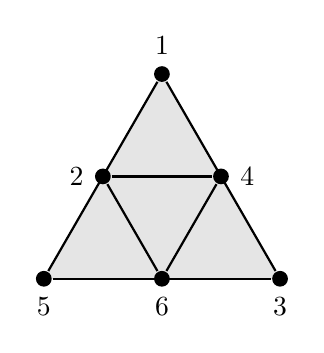
\begin{tikzpicture}[
       thick,
       acteur/.style={
         circle,
         fill=black,
         thick,
         inner sep=2pt,
         minimum size=0.2cm
       }
     ] 

	   \fill[fill=gray!20] (0,0)--(3,0)--(1.5,2.6);

       \node (a1) at (0,0) [acteur,label=below:5]{};
       \node (a2) at (3,0)[acteur,label=below:3]{}; 
       \node (a3) at (1.5,2.6) [acteur,label=above:1]{}; 
       \node (a4) at (0.75,1.3) [acteur,label=left:2]{}; 
       \node (a5) at (2.25,1.3) [acteur,label=right:4]{}; 
       \node (a6) at (1.5,0) [acteur,label=below:6]{};
  
       \draw (a1) -- (a2); 
       \draw (a2) -- (a3); 
       \draw (a1) -- (a3);
       
       \draw (a4) -- (a5);
       \draw (a5) -- (a6);
       \draw (a4) -- (a6);

\end{tikzpicture}
  \caption{The support of a $2$-Cheeger cosystole (The gray triangles represent the four $2$-simplices)}
  \label{figure1:Figure 1}
\end{figure}
